\documentclass[a4paper,12pt]{article}
\usepackage[utf8]{inputenc}
\usepackage{amsmath}
\usepackage{graphicx}
\usepackage{hyperref}
\usepackage{physics}
\usepackage{subcaption}
\usepackage{float}
\usepackage{pgffor}

\title{Aproximación de la Ecuación de Movimiento de un Péndulo Simple utilizando Redes Neuronales}
\author{Juan José González Giraldo}
\date{Mayo 2024}

\begin{document}

\maketitle

\begin{abstract}
    En este proyecto, exploramos cómo las redes neuronales pueden utilizarse para aproximar la solución de la ecuación de movimiento de un péndulo simple. El péndulo simple es un sistema físico idealizado que consiste en una masa puntual suspendida de un hilo inextensible de longitud \(L\). Diseñamos una red neuronal que predice el ángulo \(\theta\) del péndulo en función del tiempo \(t\), la longitud \(L\) y la gravedad \(g\).
\end{abstract}

\section{Introducción}
La ecuación diferencial que describe el movimiento de un péndulo simple es:
\begin{equation}
    \dv[2]{\theta}{t} + \frac{g}{L} \sin(\theta) = 0
\end{equation}
donde:
\begin{itemize}
    \item \(\theta\) es el ángulo de desplazamiento del péndulo desde la vertical,
    \item \(t\) es el tiempo,
    \item \(g\) es la aceleración debido a la gravedad,
    \item \(L\) es la longitud del péndulo.
\end{itemize}

\section{Objetivo}
Diseñar una red neuronal para aproximar la solución de la ecuación de movimiento del péndulo simple. Específicamente, la red deberá predecir el ángulo \(\theta\) del péndulo en función del tiempo \(t\), la longitud \(L\) y la gravedad \(g\).

\section{Recopilación de Datos}
La ecuación diferencial que describe el movimiento de un péndulo simple se puede solucionar como una ecuación diferencial ordinaria. Esto se expresa en la función pendulum:

\begin{verbatim}
import numpy as np
import matplotlib.pyplot as plt
from scipy.integrate import solve_ivp


# Definir la función que representa el sistema de ecuaciones diferenciales
def pendulum(t, y, L=1, g=9.81):
    theta, omega = y  # theta es el ángulo, omega es la velocidad angular
    dtheta_dt = omega
    domega_dt = -(g / L) * np.sin(theta)
    return np.array([dtheta_dt, domega_dt])
\end{verbatim}

A partir del sistema de ecuaciones diferenciales que dan soluciones a la ecuación diferencial del péndulo simple se generó un conjunto de datos con las siguientes constantes:
\begin{itemize}
    \item Rango de tiempo = [0, 10]
    \item \(g\) = \(9.81\)
    \item \(L\) = \(1\)
\end{itemize}

El conjunto de datos generado consiste en pares de entrada-salida, donde la entrada es el tiempo \(t\), y la salida es el ángulo \(\theta\) correspondiente en ese momento.

\section{Preprocesamiento de Datos}
Utilizamos normalización MinMax para transformar los datos de entrada y salida a un rango entre [0, 1]. Esto ayuda a mejorar la convergencia y estabilidad del entrenamiento. Hay que tener en cuenta que el rango de los datos de entrada al scaler determinará el rango en el que el modelo funcionará ya que valores superiores o inferiores causan valores menores que 0 y mayores que 1.

\begin{verbatim}
from sklearn.preprocessing import MinMaxScaler

# Normalizar los datos
scaler_X = MinMaxScaler()
X_normalized = scaler_X.fit_transform(X.reshape(-1, 1))

scaler_y = MinMaxScaler()
y_normalized = scaler_y.fit_transform(y.reshape(-1, 1)).flatten()
\end{verbatim}

Usamos 2 scalers para diferenciar los valores de entrada y de salida.

\section{Diseño de la Red Neuronal}
La red neuronal diseñada para este proyecto es una red feedforward (FFNN) secuencial con la siguiente arquitectura:
\begin{itemize}
    \item Capa de entrada: 1 neurona (para \(t\)).
    \item 8 capas ocultas, cada una con 64 neuronas y función de activación ReLU.
    \item Capa de salida: 1 neurona (para \(\theta\)) con función de activación lineal.
    \item Optimizador: Adam
    \item Función de pérdida: MSE
\end{itemize}

\begin{verbatim}
from tensorflow.keras.models import Sequential
from tensorflow.keras.layers import Dense, Input
from tensorflow.keras.optimizers import Adam
from tensorflow.keras.metrics import RootMeanSquaredError

model = Sequential()
model.add(Input(shape=(1,)))
model.add(Dense(64, activation="relu"))
model.add(Dense(64, activation="relu"))
model.add(Dense(64, activation="relu"))
model.add(Dense(64, activation="relu"))
model.add(Dense(64, activation="relu"))
model.add(Dense(64, activation="relu"))
model.add(Dense(64, activation="relu"))
model.add(Dense(64, activation="relu"))
model.add(Dense(1))

model.compile(optimizer=Adam(), loss="mse", metrics=[RootMeanSquaredError()])
model.summary()
\end{verbatim}

\section{Resultados}
El modelo final muestra una buena capacidad de generalización y precisión en las predicciones del ángulo \(\theta\).
\begin{itemize}
    \item MSE = \(\qty{1.21e-4}{}\)
    \item RMSE = \(\qty{6.67e-5}{}\)
\end{itemize}

\begin{figure}[H]
    \centering
    \begin{subfigure}{.7\linewidth}
        \centering
        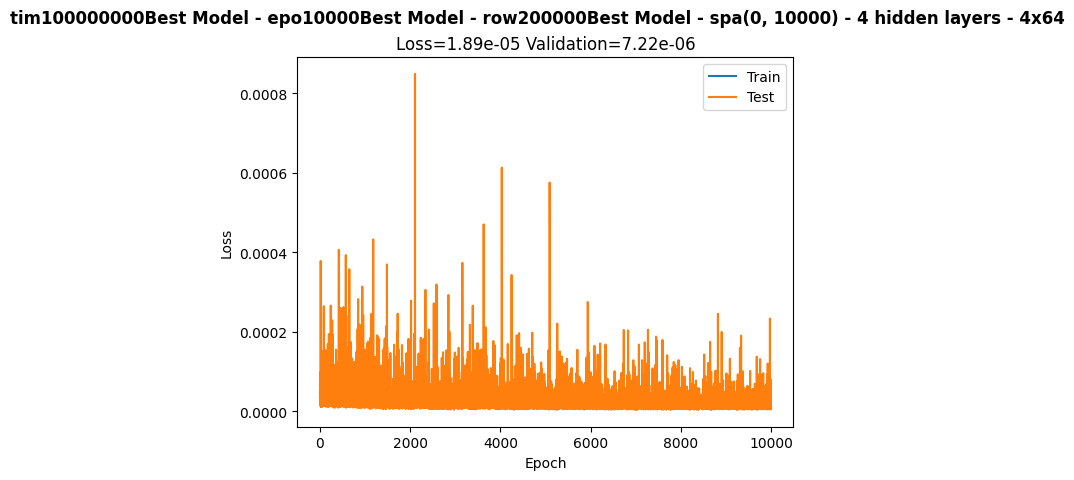
\includegraphics[width=\textwidth]{true_vs_prediction_pendulum.png}
        \caption{Reales vs predicciones en el péndulo}
        \label{fig:true_vs_prediction_pendulum}
    \end{subfigure}
    \begin{subfigure}{.7\linewidth}
        \centering
        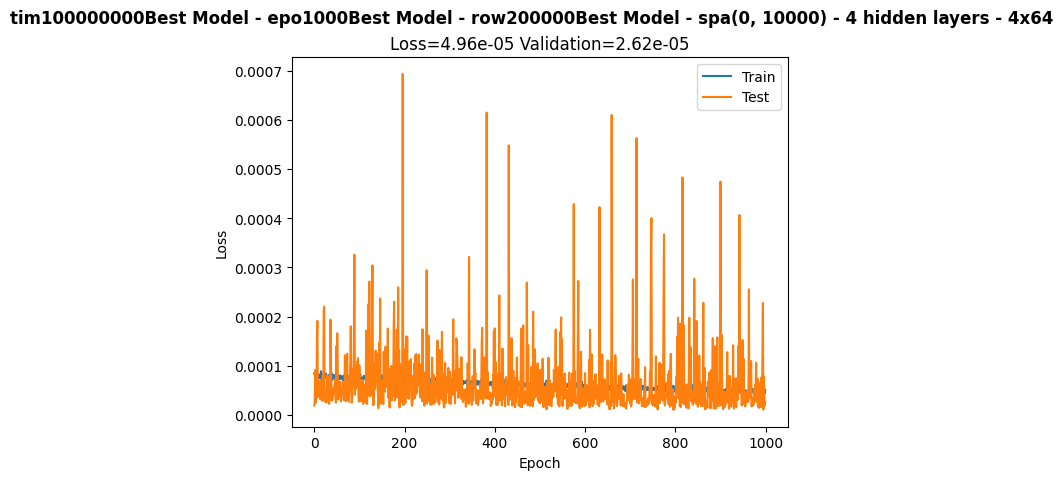
\includegraphics[width=\textwidth]{loss.png}
        \caption{Reducción del error}
        \label{fig:loss}
    \end{subfigure}
    \caption{Rendimiento del modelo}
\end{figure}

\section{Discusión}
Se entrenaron múltiples modelos variando los hiperparámetros como la cantidad de epochs, la cantidad de capas y la cantidad de neuronas en cada capa. La decisión del mejor modelo se tomó a partir del valor mas bajo de error en validación.

\subsection*{Mountain}
\begin{figure}[H]
    \centering
    \begin{subfigure}{.47\linewidth}
        \centering
        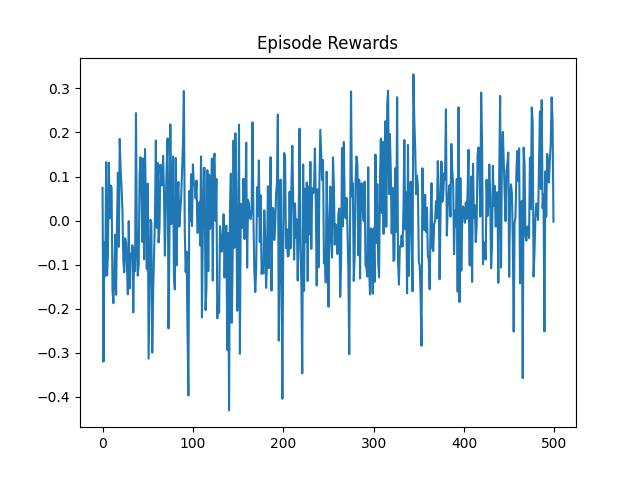
\includegraphics[width=\textwidth]{mountain/2024-06-15_08-13-32_dqn_mountaincar_episode_rewards.png}
    \end{subfigure}
    \begin{subfigure}{.47\linewidth}
        \centering
        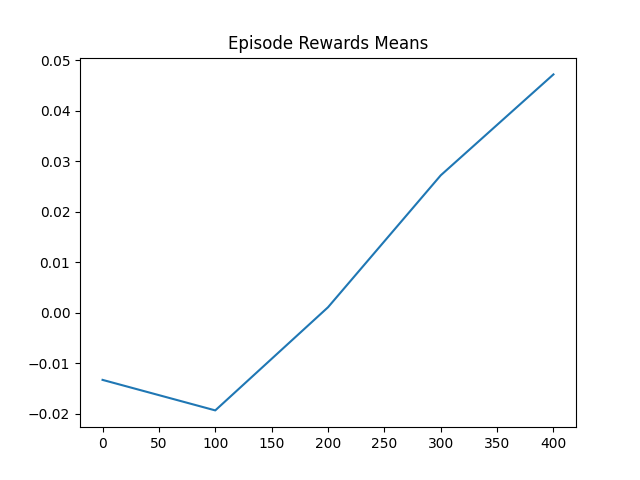
\includegraphics[width=\textwidth]{mountain/2024-06-15_08-13-32_dqn_mountaincar_episode_rewards_means.png}
    \end{subfigure}
    \begin{subfigure}{.47\linewidth}
        \centering
        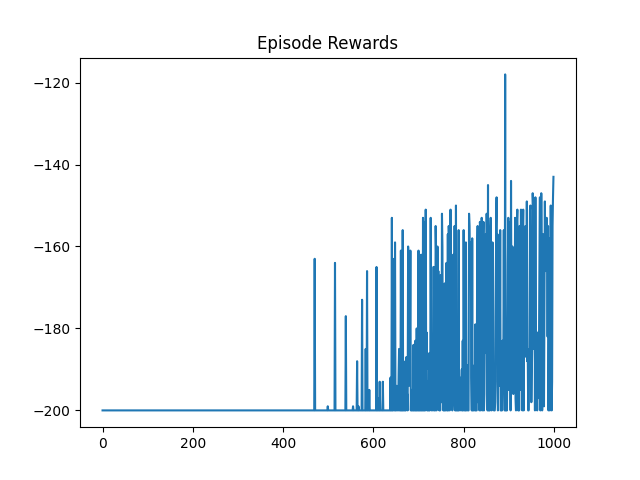
\includegraphics[width=\textwidth]{mountain/2024-06-15_10-54-10_dqn_mountaincar_episode_rewards.png}
    \end{subfigure}
    \begin{subfigure}{.47\linewidth}
        \centering
        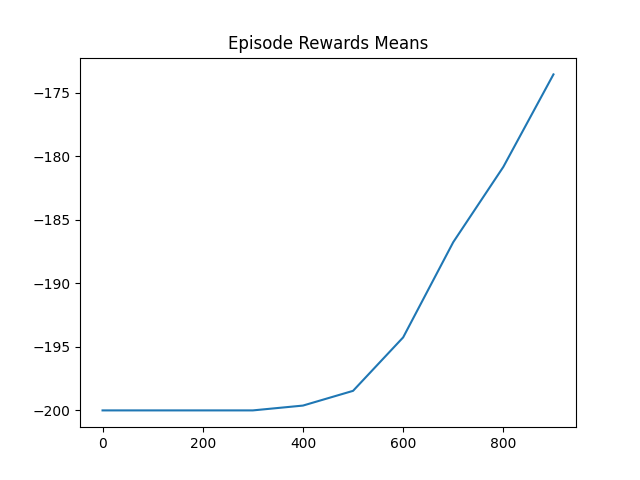
\includegraphics[width=\textwidth]{mountain/2024-06-15_10-54-10_dqn_mountaincar_episode_rewards_means.png}
    \end{subfigure}
\end{figure}
\begin{figure}[H]
    \centering
    \begin{subfigure}{.47\linewidth}
        \centering
        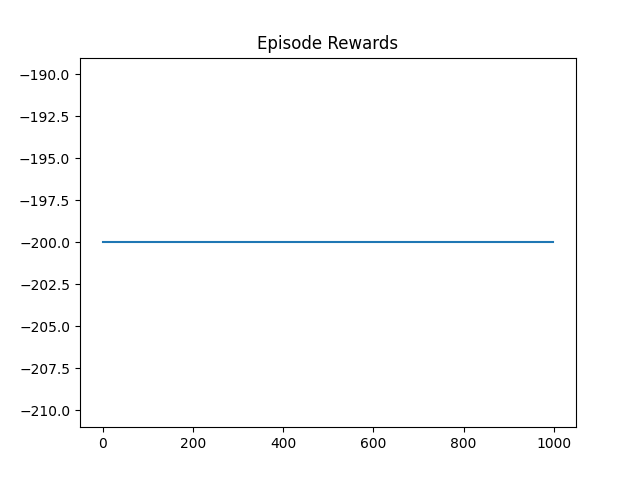
\includegraphics[width=\textwidth]{mountain/2024-06-15_11-01-53_dqn_mountaincar_episode_rewards.png}
    \end{subfigure}
    \begin{subfigure}{.47\linewidth}
        \centering
        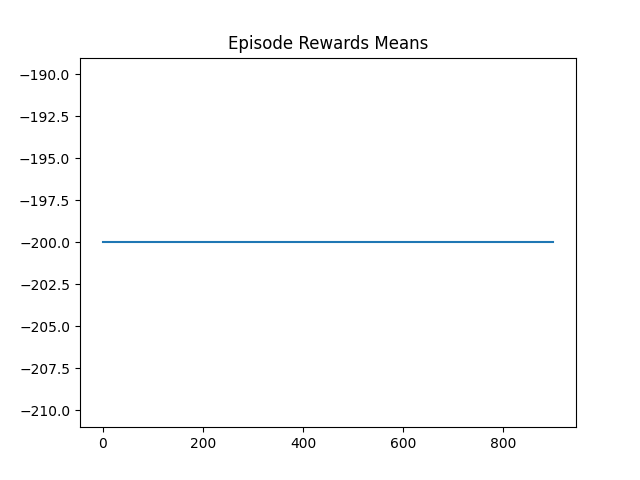
\includegraphics[width=\textwidth]{mountain/2024-06-15_11-01-53_dqn_mountaincar_episode_rewards_means.png}
    \end{subfigure}
    \begin{subfigure}{.47\linewidth}
        \centering
        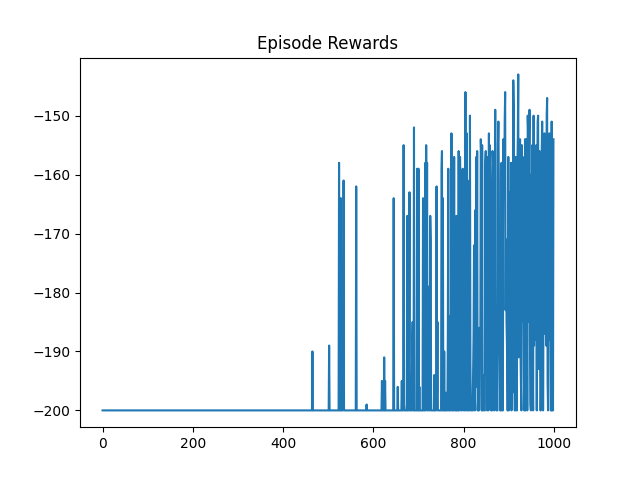
\includegraphics[width=\textwidth]{mountain/2024-06-15_11-21-25_dqn_mountaincar_episode_rewards.png}
    \end{subfigure}
    \begin{subfigure}{.47\linewidth}
        \centering
        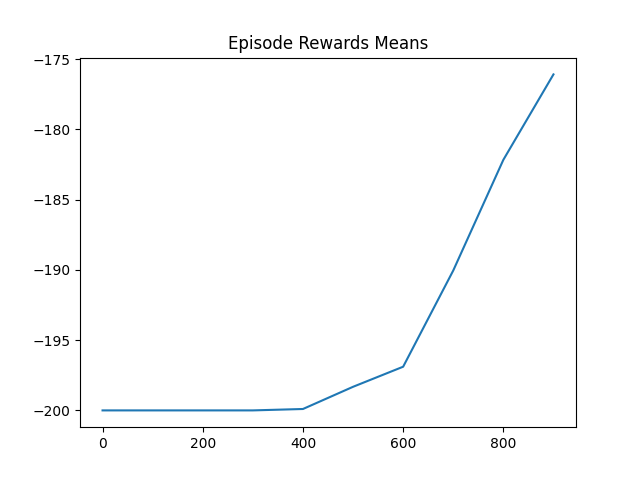
\includegraphics[width=\textwidth]{mountain/2024-06-15_11-21-25_dqn_mountaincar_episode_rewards_means.png}
    \end{subfigure}
\end{figure}
\begin{figure}[H]
    \centering
    \begin{subfigure}{.47\linewidth}
        \centering
        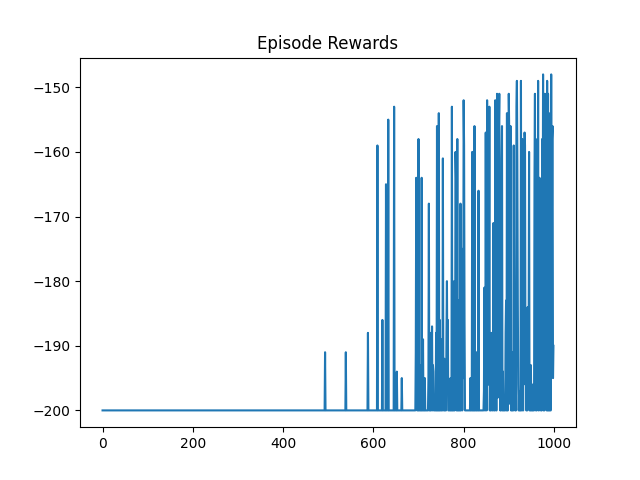
\includegraphics[width=\textwidth]{mountain/2024-06-15_11-57-24_dqn_mountaincar_episode_rewards.png}
    \end{subfigure}
    \begin{subfigure}{.47\linewidth}
        \centering
        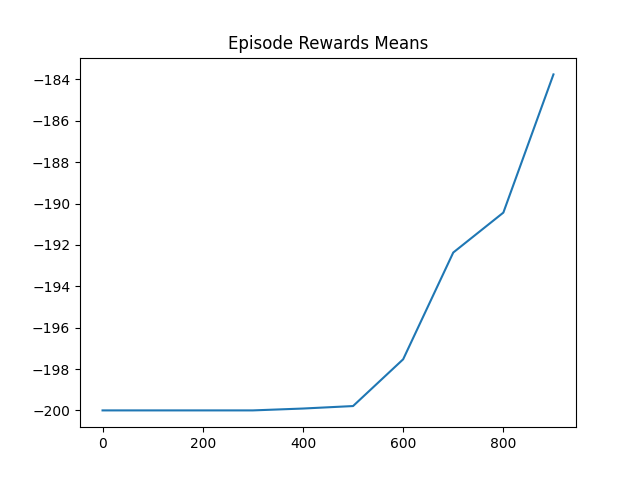
\includegraphics[width=\textwidth]{mountain/2024-06-15_11-57-24_dqn_mountaincar_episode_rewards_means.png}
    \end{subfigure}
    \begin{subfigure}{.47\linewidth}
        \centering
        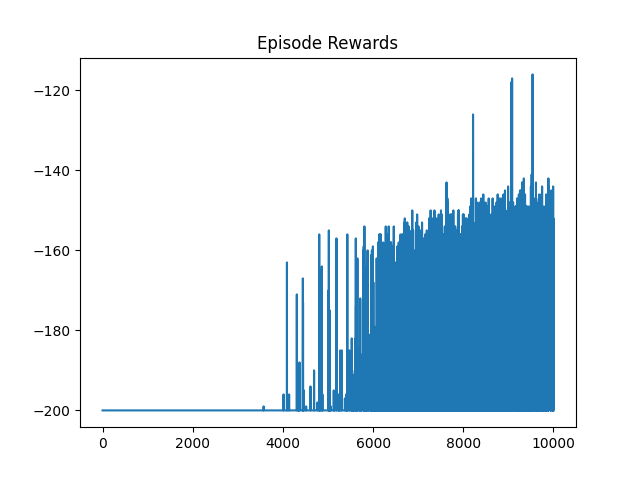
\includegraphics[width=\textwidth]{mountain/2024-06-15_12-16-56_dqn_mountaincar_episode_rewards.png}
    \end{subfigure}
    \begin{subfigure}{.47\linewidth}
        \centering
        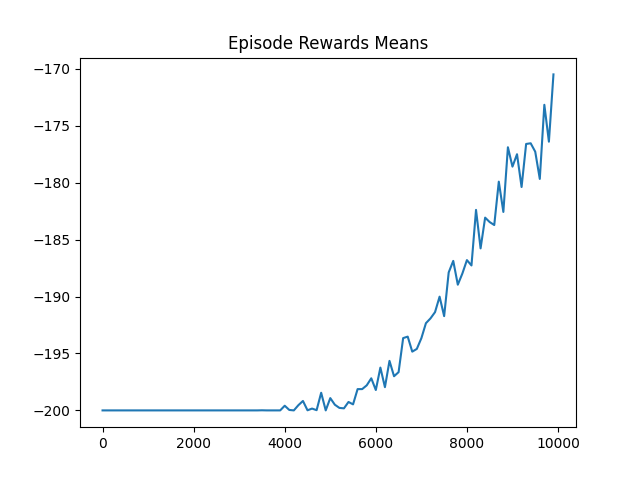
\includegraphics[width=\textwidth]{mountain/2024-06-15_12-16-56_dqn_mountaincar_episode_rewards_means.png}
    \end{subfigure}
\end{figure}
\begin{figure}[H]
    \centering
    \begin{subfigure}{.47\linewidth}
        \centering
        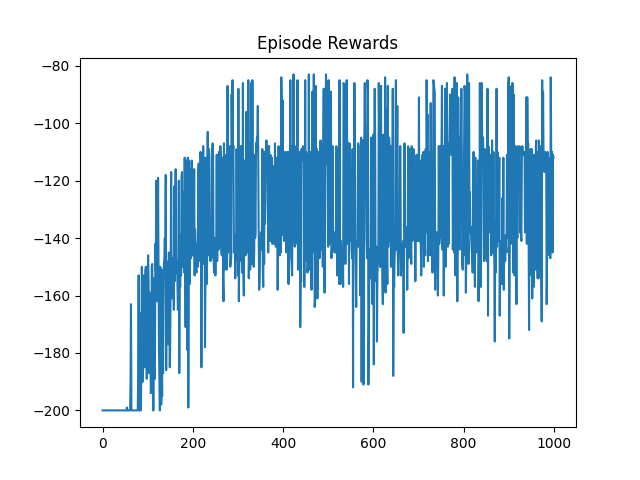
\includegraphics[width=\textwidth]{mountain/2024-06-15_12-23-27_dqn_mountaincar_episode_rewards.png}
    \end{subfigure}
    \begin{subfigure}{.47\linewidth}
        \centering
        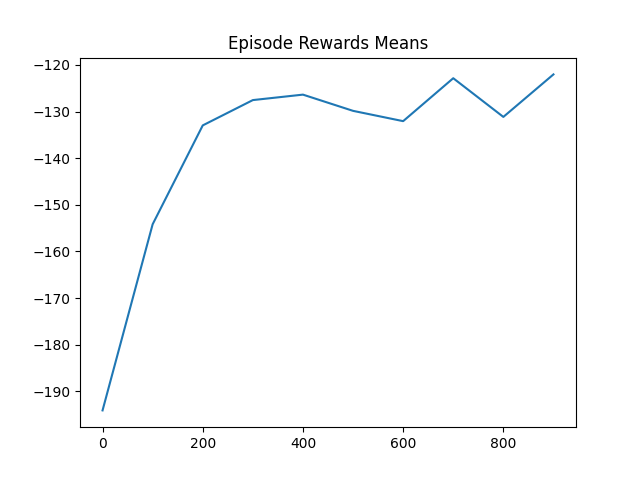
\includegraphics[width=\textwidth]{mountain/2024-06-15_12-23-27_dqn_mountaincar_episode_rewards_means.png}
    \end{subfigure}
    \begin{subfigure}{.47\linewidth}
        \centering
        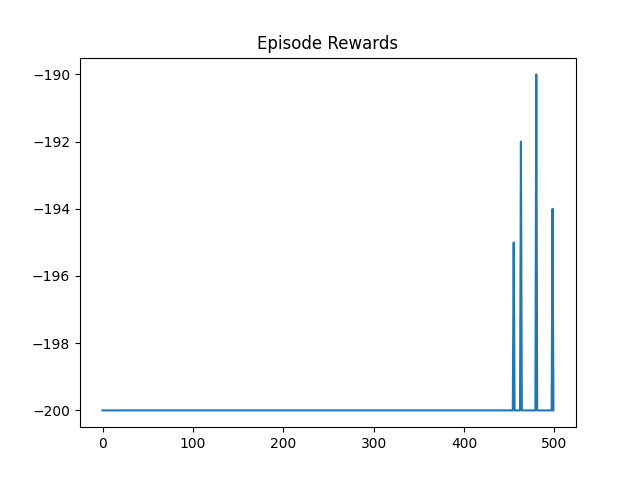
\includegraphics[width=\textwidth]{mountain/2024-06-15_12-31-16_dqn_mountaincar_episode_rewards.png}
    \end{subfigure}
    \begin{subfigure}{.47\linewidth}
        \centering
        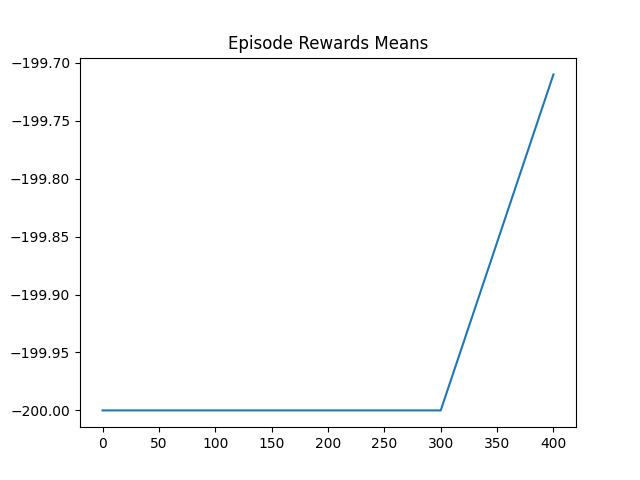
\includegraphics[width=\textwidth]{mountain/2024-06-15_12-31-16_dqn_mountaincar_episode_rewards_means.png}
    \end{subfigure}
\end{figure}
\begin{figure}[H]
    \centering
    \begin{subfigure}{.47\linewidth}
        \centering
        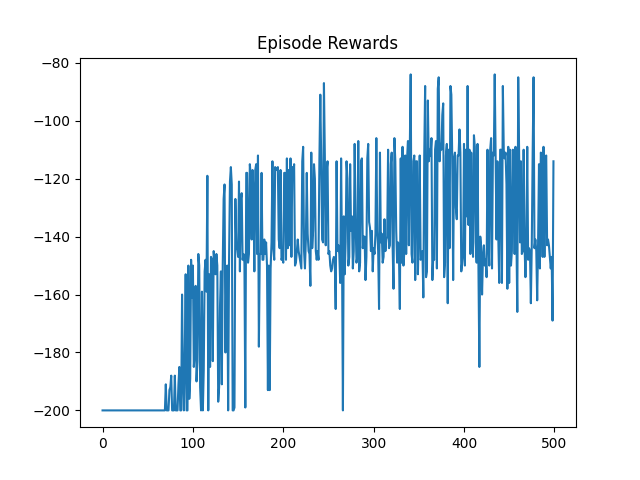
\includegraphics[width=\textwidth]{mountain/2024-06-15_12-35-51_dqn_mountaincar_episode_rewards.png}
    \end{subfigure}
    \begin{subfigure}{.47\linewidth}
        \centering
        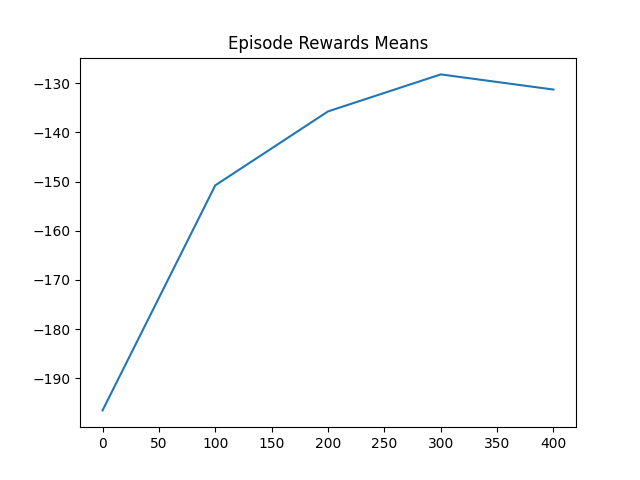
\includegraphics[width=\textwidth]{mountain/2024-06-15_12-35-51_dqn_mountaincar_episode_rewards_means.png}
    \end{subfigure}
    \begin{subfigure}{.47\linewidth}
        \centering
        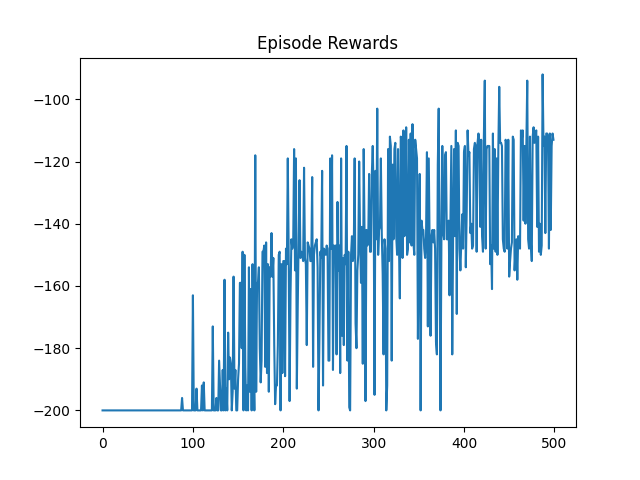
\includegraphics[width=\textwidth]{mountain/2024-06-15_12-43-21_dqn_mountaincar_episode_rewards.png}
    \end{subfigure}
    \begin{subfigure}{.47\linewidth}
        \centering
        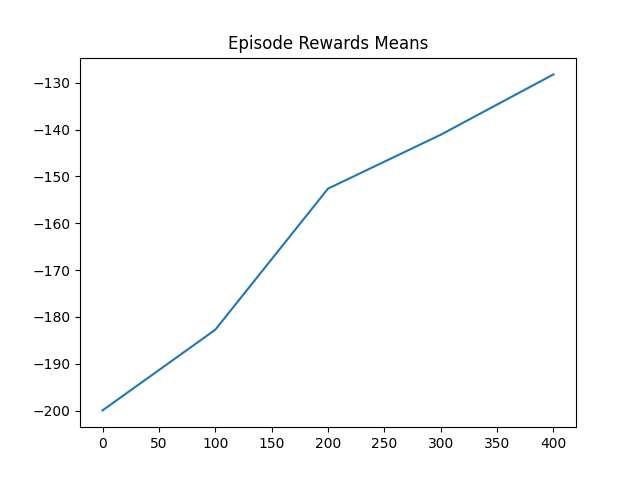
\includegraphics[width=\textwidth]{mountain/2024-06-15_12-43-21_dqn_mountaincar_episode_rewards_means.png}
    \end{subfigure}
\end{figure}
\begin{figure}[H]
    \centering
    \begin{subfigure}{.47\linewidth}
        \centering
        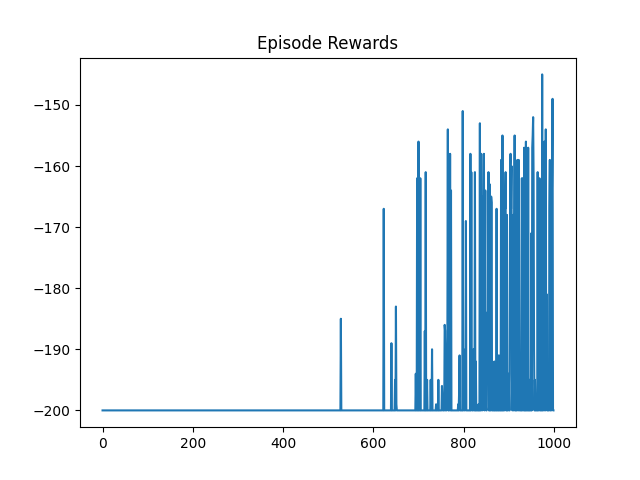
\includegraphics[width=\textwidth]{mountain/2024-06-15_12-43-26_dqn_mountaincar_episode_rewards.png}
    \end{subfigure}
    \begin{subfigure}{.47\linewidth}
        \centering
        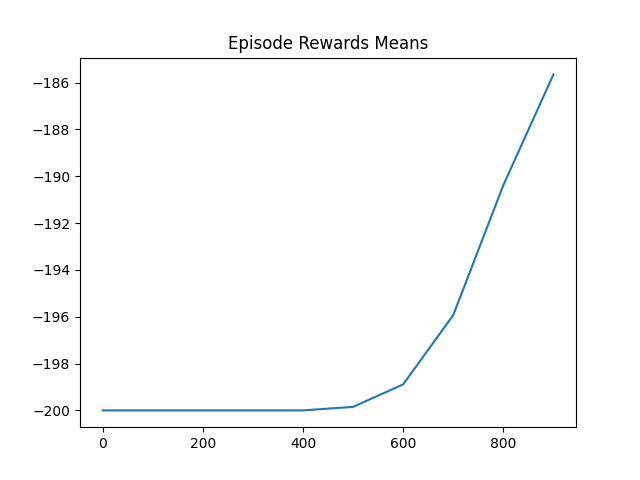
\includegraphics[width=\textwidth]{mountain/2024-06-15_12-43-26_dqn_mountaincar_episode_rewards_means.png}
    \end{subfigure}
    \begin{subfigure}{.47\linewidth}
        \centering
        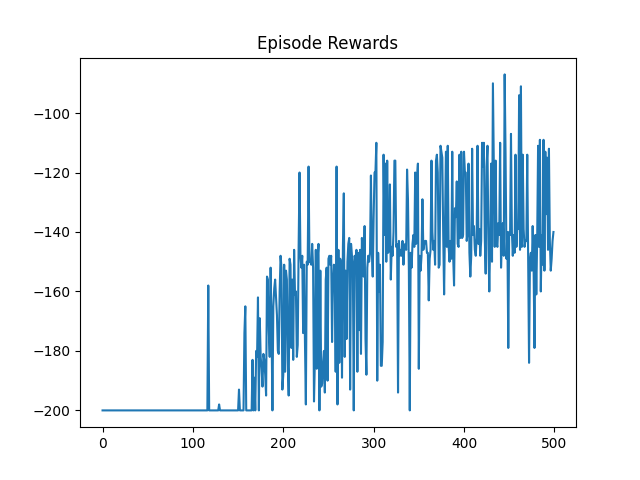
\includegraphics[width=\textwidth]{mountain/2024-06-15_13-00-05_dqn_mountaincar_episode_rewards.png}
    \end{subfigure}
    \begin{subfigure}{.47\linewidth}
        \centering
        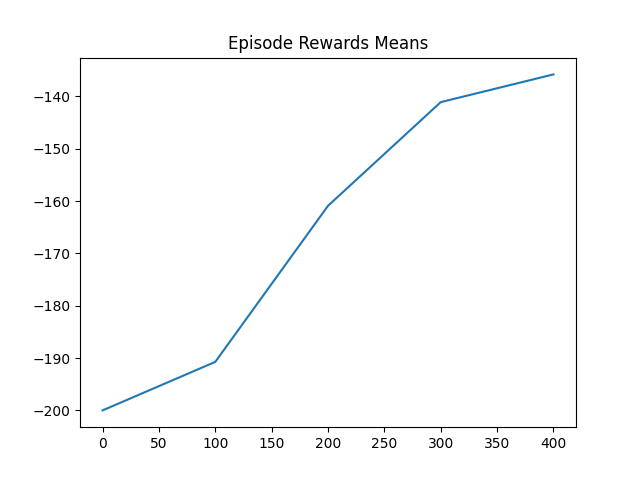
\includegraphics[width=\textwidth]{mountain/2024-06-15_13-00-05_dqn_mountaincar_episode_rewards_means.png}
    \end{subfigure}
\end{figure}
\begin{figure}[H]
    \centering
    \begin{subfigure}{.47\linewidth}
        \centering
        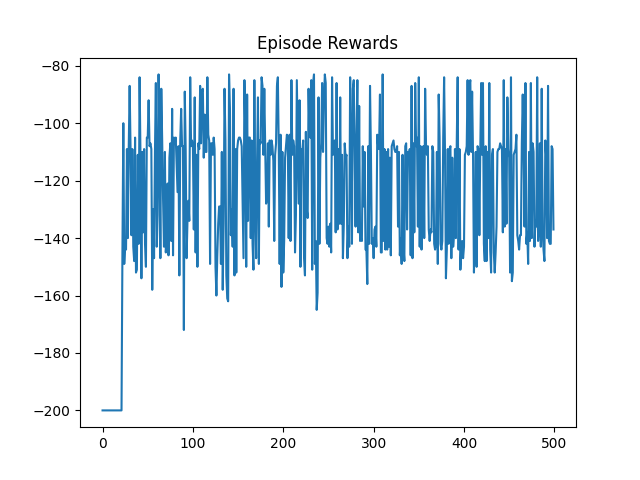
\includegraphics[width=\textwidth]{mountain/2024-06-15_13-02-52_dqn_mountaincar_episode_rewards.png}
    \end{subfigure}
    \begin{subfigure}{.47\linewidth}
        \centering
        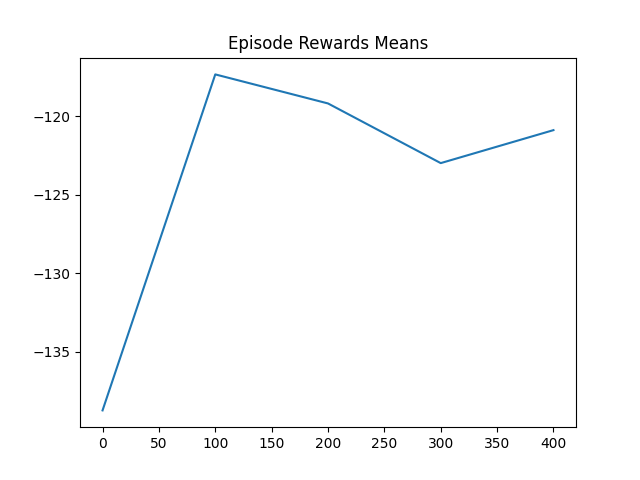
\includegraphics[width=\textwidth]{mountain/2024-06-15_13-02-52_dqn_mountaincar_episode_rewards_means.png}
    \end{subfigure}
    \begin{subfigure}{.47\linewidth}
        \centering
        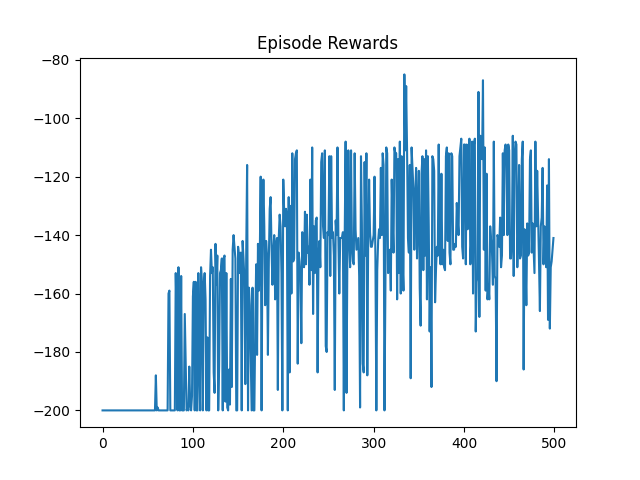
\includegraphics[width=\textwidth]{mountain/2024-06-15_13-20-27_dqn_mountaincar_episode_rewards.png}
    \end{subfigure}
    \begin{subfigure}{.47\linewidth}
        \centering
        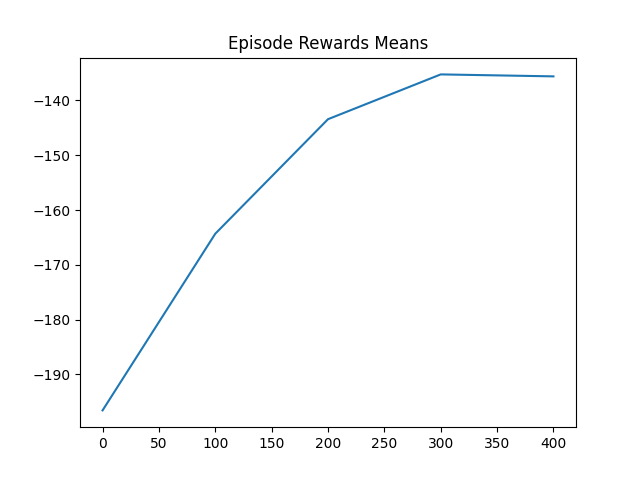
\includegraphics[width=\textwidth]{mountain/2024-06-15_13-20-27_dqn_mountaincar_episode_rewards_means.png}
    \end{subfigure}
\end{figure}
\begin{figure}[H]
    \centering
    \begin{subfigure}{.47\linewidth}
        \centering
        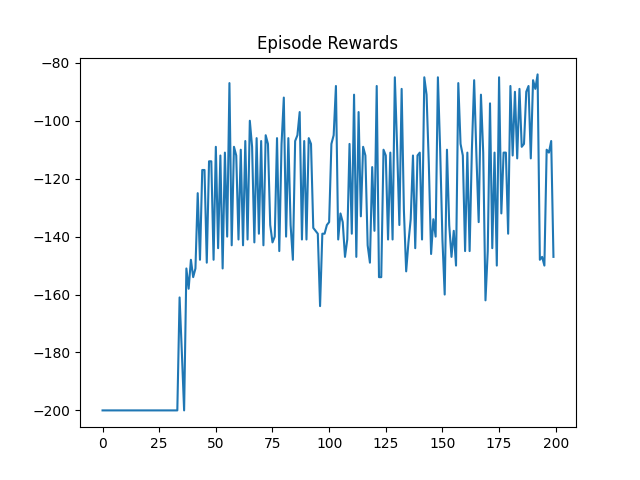
\includegraphics[width=\textwidth]{mountain/2024-06-15_13-36-42_dqn_mountaincar_episode_rewards.png}
    \end{subfigure}
    \begin{subfigure}{.47\linewidth}
        \centering
        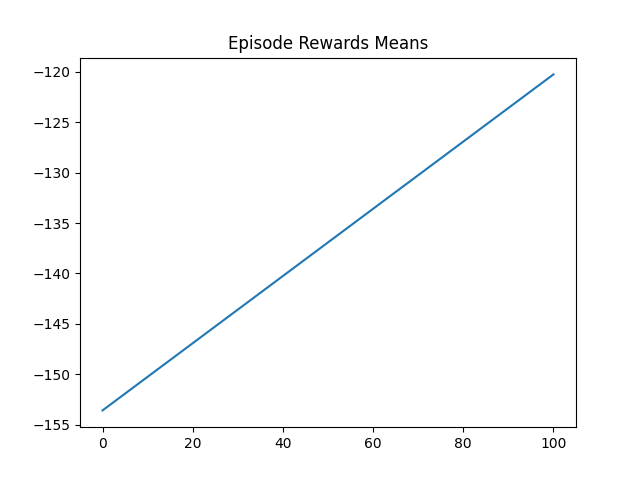
\includegraphics[width=\textwidth]{mountain/2024-06-15_13-36-42_dqn_mountaincar_episode_rewards_means.png}
    \end{subfigure}
    \begin{subfigure}{.47\linewidth}
        \centering
        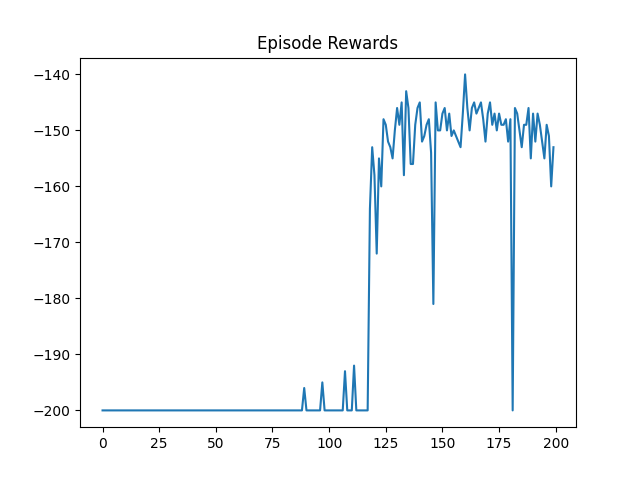
\includegraphics[width=\textwidth]{mountain/2024-06-15_13-39-22_dqn_mountaincar_episode_rewards.png}
    \end{subfigure}
    \begin{subfigure}{.47\linewidth}
        \centering
        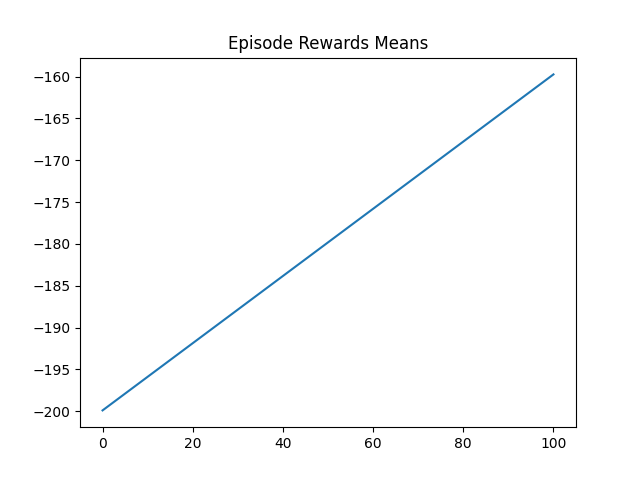
\includegraphics[width=\textwidth]{mountain/2024-06-15_13-39-22_dqn_mountaincar_episode_rewards_means.png}
    \end{subfigure}
\end{figure}
\begin{figure}[H]
    \centering
    \begin{subfigure}{.47\linewidth}
        \centering
        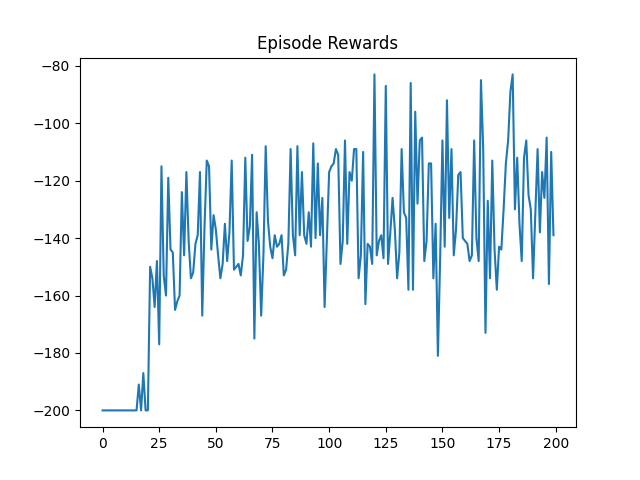
\includegraphics[width=\textwidth]{mountain/2024-06-15_13-41-53_dqn_mountaincar_episode_rewards.png}
    \end{subfigure}
    \begin{subfigure}{.47\linewidth}
        \centering
        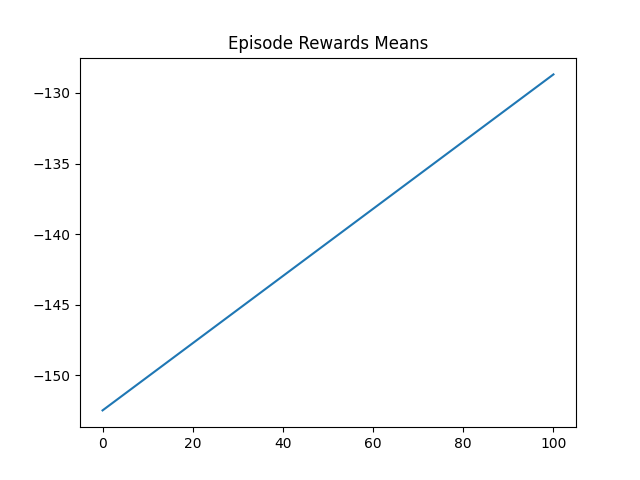
\includegraphics[width=\textwidth]{mountain/2024-06-15_13-41-53_dqn_mountaincar_episode_rewards_means.png}
    \end{subfigure}
    \begin{subfigure}{.47\linewidth}
        \centering
        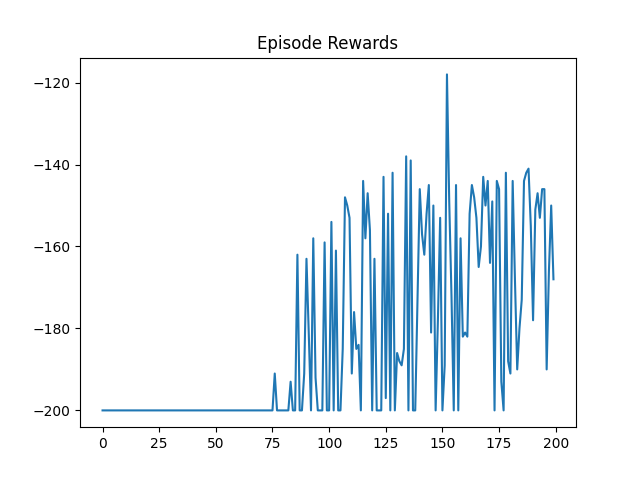
\includegraphics[width=\textwidth]{mountain/2024-06-15_13-45-28_dqn_mountaincar_episode_rewards.png}
    \end{subfigure}
    \begin{subfigure}{.47\linewidth}
        \centering
        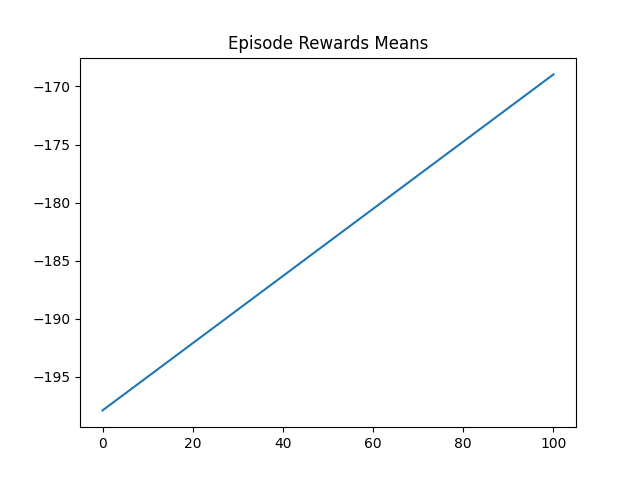
\includegraphics[width=\textwidth]{mountain/2024-06-15_13-45-28_dqn_mountaincar_episode_rewards_means.png}
    \end{subfigure}
\end{figure}
\begin{figure}[H]
    \centering
    \begin{subfigure}{.47\linewidth}
        \centering
        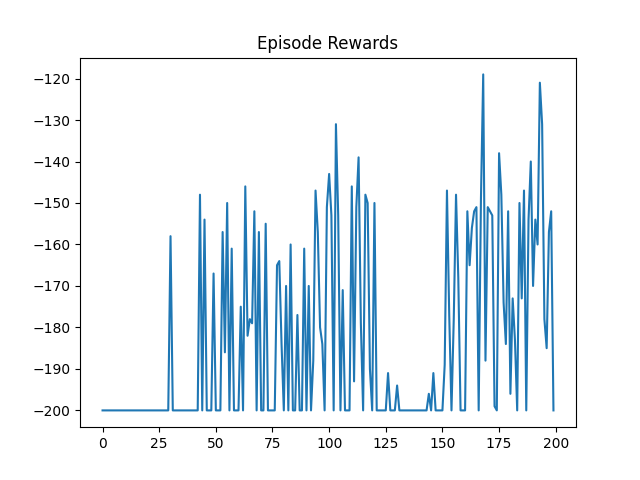
\includegraphics[width=\textwidth]{mountain/2024-06-15_13-45-47_dqn_mountaincar_episode_rewards.png}
    \end{subfigure}
    \begin{subfigure}{.47\linewidth}
        \centering
        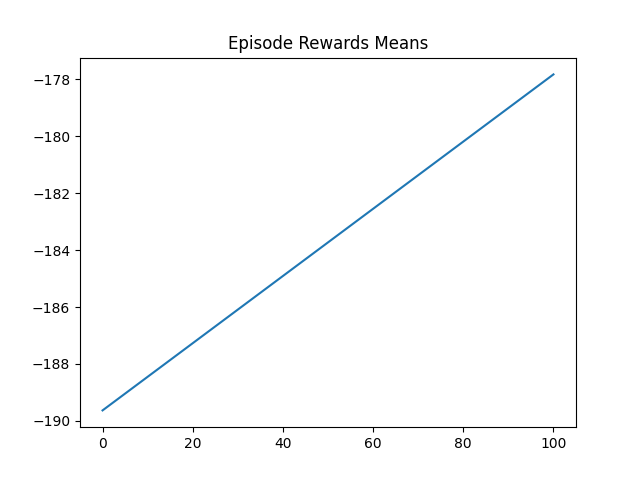
\includegraphics[width=\textwidth]{mountain/2024-06-15_13-45-47_dqn_mountaincar_episode_rewards_means.png}
    \end{subfigure}
    \begin{subfigure}{.47\linewidth}
        \centering
        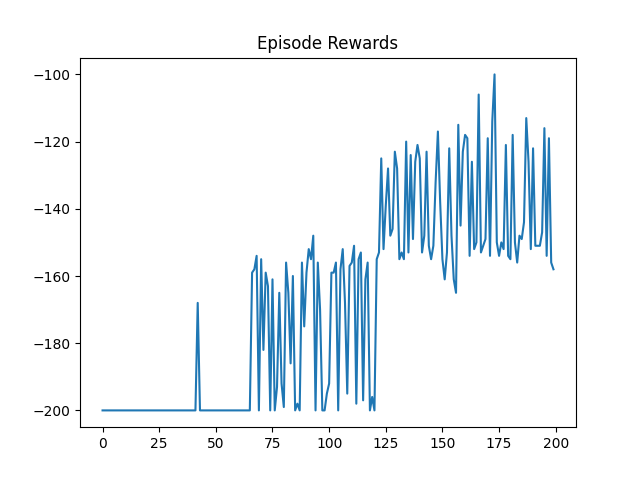
\includegraphics[width=\textwidth]{mountain/2024-06-15_13-48-51_dqn_mountaincar_episode_rewards.png}
    \end{subfigure}
    \begin{subfigure}{.47\linewidth}
        \centering
        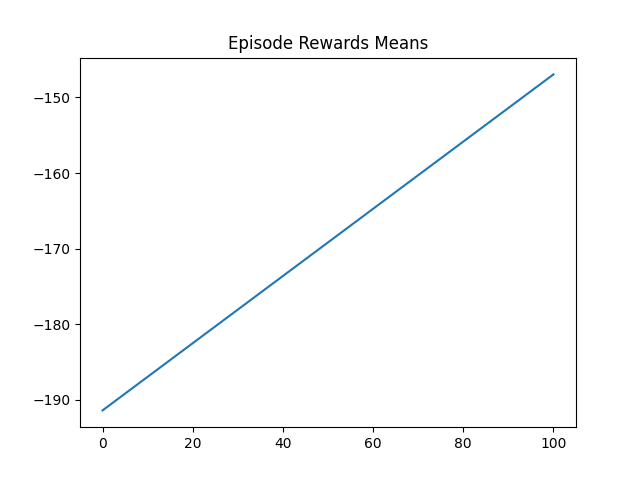
\includegraphics[width=\textwidth]{mountain/2024-06-15_13-48-51_dqn_mountaincar_episode_rewards_means.png}
    \end{subfigure}
\end{figure}
\begin{figure}[H]
    \centering
    \begin{subfigure}{.47\linewidth}
        \centering
        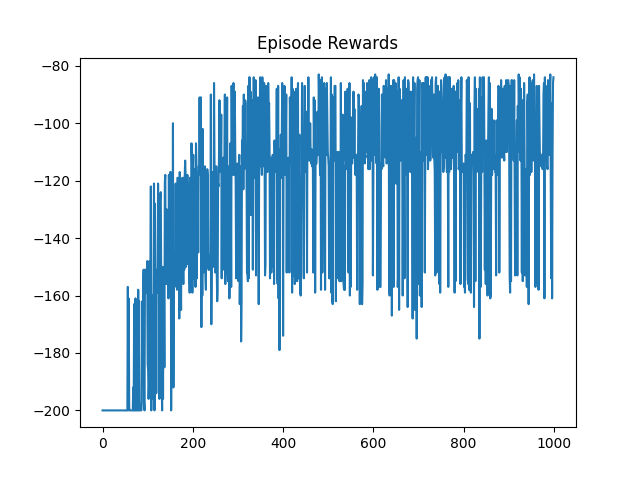
\includegraphics[width=\textwidth]{mountain/2024-06-15_13-56-21_dqn_mountaincar_episode_rewards.png}
    \end{subfigure}
    \begin{subfigure}{.47\linewidth}
        \centering
        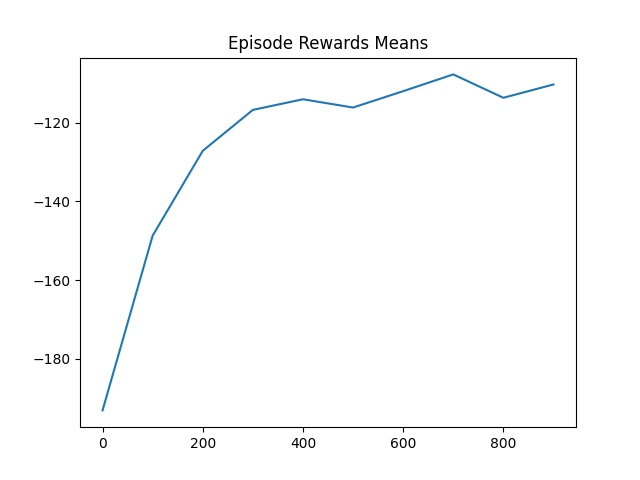
\includegraphics[width=\textwidth]{mountain/2024-06-15_13-56-21_dqn_mountaincar_episode_rewards_means.png}
    \end{subfigure}
    \begin{subfigure}{.47\linewidth}
        \centering
        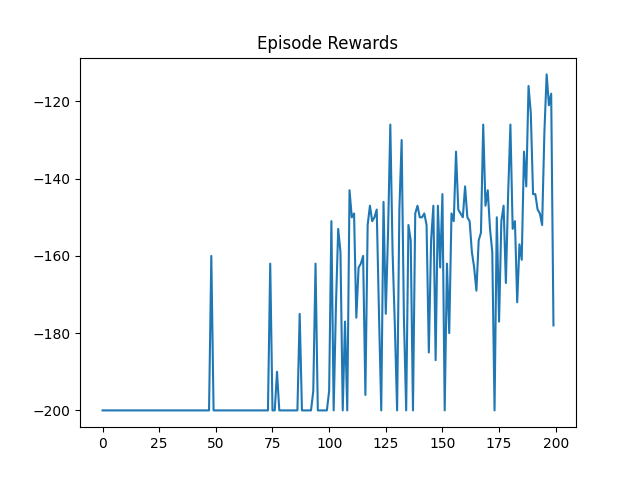
\includegraphics[width=\textwidth]{mountain/2024-06-15_16-46-16_dqn_mountaincar_episode_rewards.png}
    \end{subfigure}
    \begin{subfigure}{.47\linewidth}
        \centering
        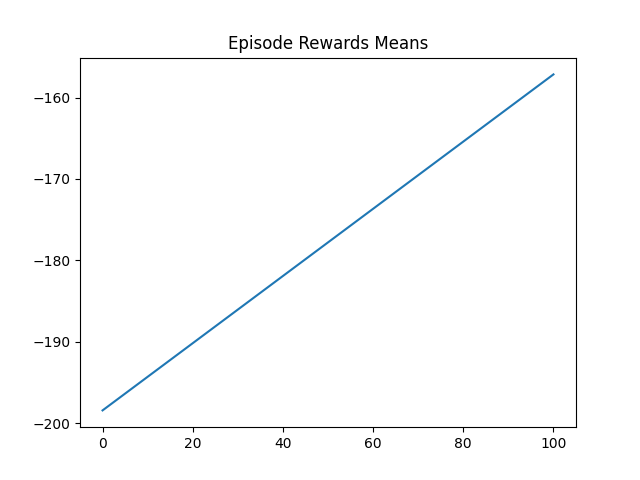
\includegraphics[width=\textwidth]{mountain/2024-06-15_16-46-16_dqn_mountaincar_episode_rewards_means.png}
    \end{subfigure}
\end{figure}


\subsection*{CartPole}
\begin{figure}[H]
    \centering
    \begin{subfigure}{.47\linewidth}
        \centering
        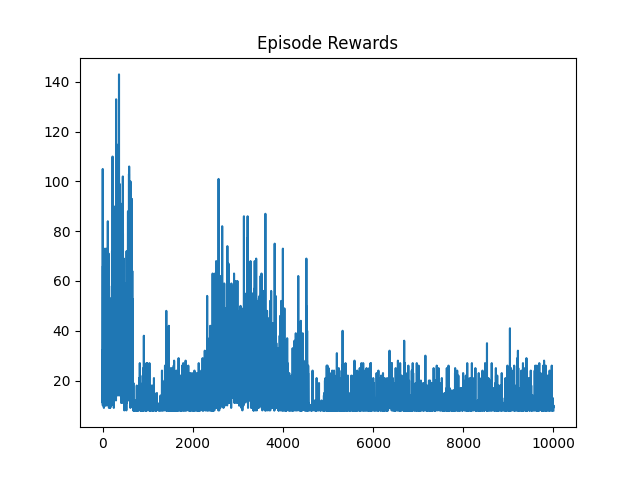
\includegraphics[width=\textwidth]{pole/2024-06-13_17-34-57_dqn_cartpole_episode_rewards.png}
    \end{subfigure}
    \begin{subfigure}{.47\linewidth}
        \centering
        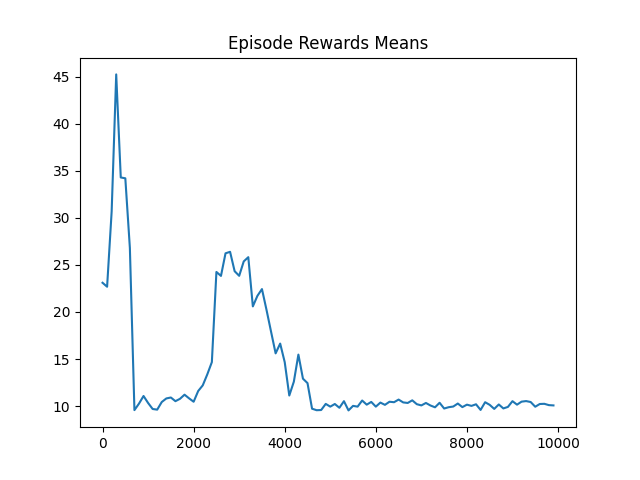
\includegraphics[width=\textwidth]{pole/2024-06-13_17-34-57_dqn_cartpole_episode_rewards_means.png}
    \end{subfigure}
    \begin{subfigure}{.47\linewidth}
        \centering
        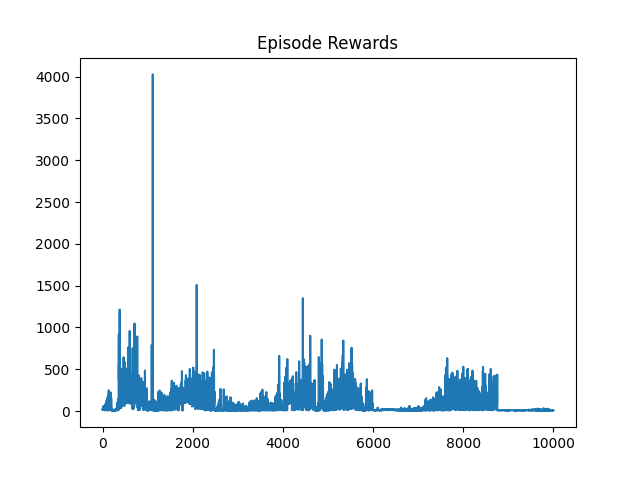
\includegraphics[width=\textwidth]{pole/2024-06-13_18-42-33_dqn_cartpole_episode_rewards.png}
    \end{subfigure}
    \begin{subfigure}{.47\linewidth}
        \centering
        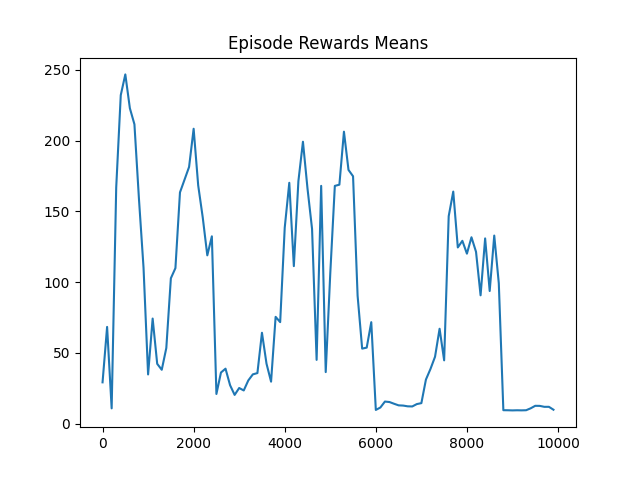
\includegraphics[width=\textwidth]{pole/2024-06-13_18-42-33_dqn_cartpole_episode_rewards_means.png}
    \end{subfigure}
\end{figure}
\begin{figure}[H]
    \centering
    \begin{subfigure}{.47\linewidth}
        \centering
        \includegraphics[width=\textwidth]{pole/2024-06-13_18-50-05_dqn_cartpole_episode_rewards.png}
    \end{subfigure}
    \begin{subfigure}{.47\linewidth}
        \centering
        \includegraphics[width=\textwidth]{pole/2024-06-13_18-50-05_dqn_cartpole_episode_rewards_means.png}
    \end{subfigure}
    \begin{subfigure}{.47\linewidth}
        \centering
        \includegraphics[width=\textwidth]{pole/2024-06-13_18-56-41_dqn_cartpole_episode_rewards.png}
    \end{subfigure}
    \begin{subfigure}{.47\linewidth}
        \centering
        \includegraphics[width=\textwidth]{pole/2024-06-13_18-56-41_dqn_cartpole_episode_rewards_means.png}
    \end{subfigure}
\end{figure}
\begin{figure}[H]
    \centering
    \begin{subfigure}{.47\linewidth}
        \centering
        \includegraphics[width=\textwidth]{pole/2024-06-13_18-59-17_dqn_cartpole_episode_rewards.png}
    \end{subfigure}
    \begin{subfigure}{.47\linewidth}
        \centering
        \includegraphics[width=\textwidth]{pole/2024-06-13_18-59-17_dqn_cartpole_episode_rewards_means.png}
    \end{subfigure}
    \begin{subfigure}{.47\linewidth}
        \centering
        \includegraphics[width=\textwidth]{pole/2024-06-13_19-11-27_dqn_cartpole_episode_rewards.png}
    \end{subfigure}
    \begin{subfigure}{.47\linewidth}
        \centering
        \includegraphics[width=\textwidth]{pole/2024-06-13_19-11-27_dqn_cartpole_episode_rewards_means.png}
    \end{subfigure}
\end{figure}
\begin{figure}[H]
    \centering
    \begin{subfigure}{.47\linewidth}
        \centering
        \includegraphics[width=\textwidth]{pole/2024-06-13_19-16-11_dqn_cartpole_episode_rewards.png}
    \end{subfigure}
    \begin{subfigure}{.47\linewidth}
        \centering
        \includegraphics[width=\textwidth]{pole/2024-06-13_19-16-11_dqn_cartpole_episode_rewards_means.png}
    \end{subfigure}
    \begin{subfigure}{.47\linewidth}
        \centering
        \includegraphics[width=\textwidth]{pole/2024-06-13_19-37-45_dqn_cartpole_episode_rewards.png}
    \end{subfigure}
    \begin{subfigure}{.47\linewidth}
        \centering
        \includegraphics[width=\textwidth]{pole/2024-06-13_19-37-45_dqn_cartpole_episode_rewards_means.png}
    \end{subfigure}
\end{figure}
\begin{figure}[H]
    \centering
    \begin{subfigure}{.47\linewidth}
        \centering
        \includegraphics[width=\textwidth]{pole/2024-06-13_20-39-12_dqn_cartpole_episode_rewards.png}
    \end{subfigure}
    \begin{subfigure}{.47\linewidth}
        \centering
        \includegraphics[width=\textwidth]{pole/2024-06-13_20-39-12_dqn_cartpole_episode_rewards_means.png}
    \end{subfigure}
    \begin{subfigure}{.47\linewidth}
        \centering
        \includegraphics[width=\textwidth]{pole/2024-06-13_21-08-24_dqn_cartpole_episode_rewards.png}
    \end{subfigure}
    \begin{subfigure}{.47\linewidth}
        \centering
        \includegraphics[width=\textwidth]{pole/2024-06-13_21-08-24_dqn_cartpole_episode_rewards_means.png}
    \end{subfigure}
\end{figure}
\begin{figure}[H]
    \centering
    \begin{subfigure}{.47\linewidth}
        \centering
        \includegraphics[width=\textwidth]{pole/2024-06-13_21-45-52_dqn_cartpole_episode_rewards.png}
    \end{subfigure}
    \begin{subfigure}{.47\linewidth}
        \centering
        \includegraphics[width=\textwidth]{pole/2024-06-13_21-45-52_dqn_cartpole_episode_rewards_means.png}
    \end{subfigure}
    \begin{subfigure}{.47\linewidth}
        \centering
        \includegraphics[width=\textwidth]{pole/2024-06-13_22-09-48_dqn_cartpole_episode_rewards.png}
    \end{subfigure}
    \begin{subfigure}{.47\linewidth}
        \centering
        \includegraphics[width=\textwidth]{pole/2024-06-13_22-09-48_dqn_cartpole_episode_rewards_means.png}
    \end{subfigure}
\end{figure}
\begin{figure}[H]
    \centering
    \begin{subfigure}{.47\linewidth}
        \centering
        \includegraphics[width=\textwidth]{pole/2024-06-13_22-34-12_dqn_cartpole_episode_rewards.png}
    \end{subfigure}
    \begin{subfigure}{.47\linewidth}
        \centering
        \includegraphics[width=\textwidth]{pole/2024-06-13_22-34-12_dqn_cartpole_episode_rewards_means.png}
    \end{subfigure}
    \begin{subfigure}{.47\linewidth}
        \centering
        \includegraphics[width=\textwidth]{pole/2024-06-13_23-08-40_dqn_cartpole_episode_rewards.png}
    \end{subfigure}
    \begin{subfigure}{.47\linewidth}
        \centering
        \includegraphics[width=\textwidth]{pole/2024-06-13_23-08-40_dqn_cartpole_episode_rewards_means.png}
    \end{subfigure}
\end{figure}
\begin{figure}[H]
    \centering
    \begin{subfigure}{.47\linewidth}
        \centering
        \includegraphics[width=\textwidth]{pole/2024-06-13_23-49-30_dqn_cartpole_episode_rewards.png}
    \end{subfigure}
    \begin{subfigure}{.47\linewidth}
        \centering
        \includegraphics[width=\textwidth]{pole/2024-06-13_23-49-30_dqn_cartpole_episode_rewards_means.png}
    \end{subfigure}
    \begin{subfigure}{.47\linewidth}
        \centering
        \includegraphics[width=\textwidth]{pole/2024-06-14_00-20-45_dqn_cartpole_episode_rewards.png}
    \end{subfigure}
    \begin{subfigure}{.47\linewidth}
        \centering
        \includegraphics[width=\textwidth]{pole/2024-06-14_00-20-45_dqn_cartpole_episode_rewards_means.png}
    \end{subfigure}
\end{figure}
\begin{figure}[H]
    \centering
    \begin{subfigure}{.47\linewidth}
        \centering
        \includegraphics[width=\textwidth]{pole/2024-06-14_09-34-50_dqn_cartpole_episode_rewards.png}
    \end{subfigure}
    \begin{subfigure}{.47\linewidth}
        \centering
        \includegraphics[width=\textwidth]{pole/2024-06-14_09-34-50_dqn_cartpole_episode_rewards_means.png}
    \end{subfigure}
    \begin{subfigure}{.47\linewidth}
        \centering
        \includegraphics[width=\textwidth]{pole/2024-06-14_11-09-14_dqn_cartpole_episode_rewards.png}
    \end{subfigure}
    \begin{subfigure}{.47\linewidth}
        \centering
        \includegraphics[width=\textwidth]{pole/2024-06-14_11-09-14_dqn_cartpole_episode_rewards_means.png}
    \end{subfigure}
\end{figure}
\begin{figure}[H]
    \centering
    \begin{subfigure}{.47\linewidth}
        \centering
        \includegraphics[width=\textwidth]{pole/2024-06-14_13-15-56_dqn_cartpole_episode_rewards.png}
    \end{subfigure}
    \begin{subfigure}{.47\linewidth}
        \centering
        \includegraphics[width=\textwidth]{pole/2024-06-14_13-15-56_dqn_cartpole_episode_rewards_means.png}
    \end{subfigure}
    \begin{subfigure}{.47\linewidth}
        \centering
        \includegraphics[width=\textwidth]{pole/2024-06-14_13-24-09_dqn_cartpole_episode_rewards.png}
    \end{subfigure}
    \begin{subfigure}{.47\linewidth}
        \centering
        \includegraphics[width=\textwidth]{pole/2024-06-14_13-24-09_dqn_cartpole_episode_rewards_means.png}
    \end{subfigure}
\end{figure}
\begin{figure}[H]
    \centering
    \begin{subfigure}{.47\linewidth}
        \centering
        \includegraphics[width=\textwidth]{pole/2024-06-14_15-38-10_dqn_cartpole_episode_rewards.png}
    \end{subfigure}
    \begin{subfigure}{.47\linewidth}
        \centering
        \includegraphics[width=\textwidth]{pole/2024-06-14_15-38-10_dqn_cartpole_episode_rewards_means.png}
    \end{subfigure}
    \begin{subfigure}{.47\linewidth}
        \centering
        \includegraphics[width=\textwidth]{pole/2024-06-14_16-42-26_dqn_cartpole_episode_rewards.png}
    \end{subfigure}
    \begin{subfigure}{.47\linewidth}
        \centering
        \includegraphics[width=\textwidth]{pole/2024-06-14_16-42-26_dqn_cartpole_episode_rewards_means.png}
    \end{subfigure}
\end{figure}
\begin{figure}[H]
    \centering
    \begin{subfigure}{.47\linewidth}
        \centering
        \includegraphics[width=\textwidth]{pole/2024-06-14_17-21-25_dqn_cartpole_episode_rewards.png}
    \end{subfigure}
    \begin{subfigure}{.47\linewidth}
        \centering
        \includegraphics[width=\textwidth]{pole/2024-06-14_17-21-25_dqn_cartpole_episode_rewards_means.png}
    \end{subfigure}
    \begin{subfigure}{.47\linewidth}
        \centering
        \includegraphics[width=\textwidth]{pole/2024-06-14_17-31-42_dqn_cartpole_episode_rewards.png}
    \end{subfigure}
    \begin{subfigure}{.47\linewidth}
        \centering
        \includegraphics[width=\textwidth]{pole/2024-06-14_17-31-42_dqn_cartpole_episode_rewards_means.png}
    \end{subfigure}
\end{figure}
\begin{figure}[H]
    \centering
    \begin{subfigure}{.47\linewidth}
        \centering
        \includegraphics[width=\textwidth]{pole/2024-06-14_18-05-51_dqn_cartpole_episode_rewards.png}
    \end{subfigure}
    \begin{subfigure}{.47\linewidth}
        \centering
        \includegraphics[width=\textwidth]{pole/2024-06-14_18-05-51_dqn_cartpole_episode_rewards_means.png}
    \end{subfigure}
    \begin{subfigure}{.47\linewidth}
        \centering
        \includegraphics[width=\textwidth]{pole/2024-06-14_18-17-10_dqn_cartpole_episode_rewards.png}
    \end{subfigure}
    \begin{subfigure}{.47\linewidth}
        \centering
        \includegraphics[width=\textwidth]{pole/2024-06-14_18-17-10_dqn_cartpole_episode_rewards_means.png}
    \end{subfigure}
\end{figure}
\begin{figure}[H]
    \centering
    \begin{subfigure}{.47\linewidth}
        \centering
        \includegraphics[width=\textwidth]{pole/2024-06-14_18-50-42_dqn_cartpole_episode_rewards.png}
    \end{subfigure}
    \begin{subfigure}{.47\linewidth}
        \centering
        \includegraphics[width=\textwidth]{pole/2024-06-14_18-50-42_dqn_cartpole_episode_rewards_means.png}
    \end{subfigure}
    \begin{subfigure}{.47\linewidth}
        \centering
        \includegraphics[width=\textwidth]{pole/2024-06-14_18-54-27_dqn_cartpole_episode_rewards.png}
    \end{subfigure}
    \begin{subfigure}{.47\linewidth}
        \centering
        \includegraphics[width=\textwidth]{pole/2024-06-14_18-54-27_dqn_cartpole_episode_rewards_means.png}
    \end{subfigure}
\end{figure}
\begin{figure}[H]
    \centering
    \begin{subfigure}{.47\linewidth}
        \centering
        \includegraphics[width=\textwidth]{pole/2024-06-14_19-20-40_dqn_cartpole_episode_rewards.png}
    \end{subfigure}
    \begin{subfigure}{.47\linewidth}
        \centering
        \includegraphics[width=\textwidth]{pole/2024-06-14_19-20-40_dqn_cartpole_episode_rewards_means.png}
    \end{subfigure}
    \begin{subfigure}{.47\linewidth}
        \centering
        \includegraphics[width=\textwidth]{pole/2024-06-15_00-29-02_dqn_cartpole_episode_rewards.png}
    \end{subfigure}
    \begin{subfigure}{.47\linewidth}
        \centering
        \includegraphics[width=\textwidth]{pole/2024-06-15_00-29-02_dqn_cartpole_episode_rewards_means.png}
    \end{subfigure}
\end{figure}


\section{Conclusión}
Concluimos que las redes neuronales pueden ser una herramienta eficaz para aproximar la solución de la ecuación de movimiento de un péndulo simple. Sin embargo, es importante considerar la complejidad del modelo y la calidad de los datos de entrada para obtener resultados precisos.

\end{document}
